\pdfinfoomitdate=1
\pdfsuppressptexinfo=15
\pdftrailerid{}
\documentclass[11pt,a4paper]{report}

\usepackage[margin=25mm,headheight=22pt]{geometry}
\usepackage[T1]{fontenc}
\usepackage[utf8]{inputenc}
\usepackage{lmodern}
\usepackage{microtype}
\usepackage{graphicx}
\usepackage{booktabs}
\usepackage{longtable}
\usepackage{tabularx}
\usepackage{array}
\usepackage{enumitem}
\usepackage{xcolor}
\usepackage{fancyhdr}
\usepackage{titlesec}
\usepackage{tikz}
\usepackage{listings}
\usepackage{setspace}
\usepackage{hyperref}
\usetikzlibrary{arrows.meta,positioning,shapes.geometric,fit}

\definecolor{VisionBlue}{HTML}{146EF5}
\definecolor{Ink}{HTML}{172033}
\definecolor{Muted}{HTML}{5E6878}
\definecolor{Rule}{HTML}{D9DEE7}
\definecolor{SoftBlue}{HTML}{EAF2FF}
\definecolor{SoftGreen}{HTML}{EAF7F1}
\definecolor{CodeBg}{HTML}{F5F7FA}

\hypersetup{
  colorlinks=true,
  linkcolor=Ink,
  urlcolor=VisionBlue,
  citecolor=VisionBlue,
  pdftitle={VisionX Project Report},
  pdfauthor={Suryadeep Singh Deswal},
  pdfsubject={Public X feed sharing Chrome extension and backend API},
  pdfkeywords={VisionX, Chrome Extension, Flask, PostgreSQL, OAuth, X API}
}

\setstretch{1.12}
\setlength{\parindent}{0pt}
\setlength{\parskip}{0.55em}
\setlist[itemize]{leftmargin=1.5em,itemsep=0.2em,topsep=0.3em}
\setlist[enumerate]{leftmargin=1.7em,itemsep=0.25em,topsep=0.3em}
\renewcommand{\arraystretch}{1.25}
\raggedbottom

\titleformat{\chapter}[display]
  {\normalfont\bfseries\color{Ink}}
  {\color{VisionBlue}\large Chapter \thechapter}
  {0.3em}
  {\Huge}
\titlespacing*{\chapter}{0pt}{-12pt}{22pt}
\titleformat{\section}{\Large\bfseries\color{Ink}}{\thesection}{0.7em}{}
\titleformat{\subsection}{\large\bfseries\color{Ink}}{\thesubsection}{0.7em}{}

\pagestyle{fancy}
\fancyhf{}
\fancyhead[L]{\small\color{Muted}VisionX Project Report}
\fancyhead[R]{\small\color{Muted}Suryadeep Singh Deswal}
\fancyfoot[C]{\small\thepage}
\renewcommand{\headrulewidth}{0.4pt}
\renewcommand{\headrule}{\hbox to\headwidth{\color{Rule}\leaders\hrule height \headrulewidth\hfill}}

\fancypagestyle{plain}{
  \fancyhf{}
  \fancyfoot[C]{\small\thepage}
  \renewcommand{\headrulewidth}{0pt}
}

\newcolumntype{Y}{>{\raggedright\arraybackslash}X}
\newcolumntype{L}[1]{>{\raggedright\arraybackslash}p{#1}}

\lstdefinestyle{visionx}{
  backgroundcolor=\color{CodeBg},
  basicstyle=\ttfamily\small,
  breaklines=true,
  frame=single,
  rulecolor=\color{Rule},
  showstringspaces=false,
  columns=fullflexible,
  keepspaces=true,
  xleftmargin=0.5em,
  xrightmargin=0.5em,
  aboveskip=0.7em,
  belowskip=0.7em
}

\newcommand{\code}[1]{\texttt{#1}}
\newcommand{\api}[2]{\texttt{#1} \texttt{#2}}

\begin{document}

\hypersetup{pageanchor=false}
\begin{titlepage}
  \thispagestyle{empty}
  \begin{tikzpicture}[remember picture,overlay]
    \fill[Ink] (current page.north west) rectangle ([yshift=-100mm]current page.north east);
    \fill[VisionBlue] ([yshift=-100mm]current page.north west)
      rectangle ([yshift=-103mm]current page.north east);
  \end{tikzpicture}

  \vspace*{8mm}
  \begin{center}
    {\fontsize{36}{42}\selectfont\bfseries\color{white} VisionX\par}
    \vspace{3mm}
    {\Large\color{white} Public X Feed Sharing Extension and Backend\par}
    \vspace{8mm}
    
\includegraphics[width=24mm]{../extension/assets/icon-128.png}
  \end{center}

  \vspace{24mm}
  \begin{center}
    {\LARGE\bfseries\color{Ink} Project Report\par}
    \vspace{10mm}
    {\large\color{Muted}
      Design, implementation, security, testing, and deployment readiness\par}
  \end{center}

  \vfill
  \begin{center}
    \color{Rule}\rule{0.55\textwidth}{0.6pt}

    \vspace{7mm}
    {\large\bfseries\color{Ink} Author: Suryadeep Singh Deswal\par}
    \vspace{7mm}
    \color{Rule}\rule{0.55\textwidth}{0.6pt}
  \end{center}
  \vspace*{12mm}
\end{titlepage}

\hypersetup{pageanchor=true}
\pagenumbering{roman}

\chapter*{Project Declaration}
\addcontentsline{toc}{chapter}{Project Declaration}
I developed VisionX as an end-to-end software project consisting of a browser
extension, a web API, a relational database, deployment configuration, and an
automated test pipeline. The implementation described in this report is the
implementation contained in the accompanying repository.

My work covered the complete flow: account creation, secure session handling,
X account verification, controlled feed sharing, retrieval of public posts,
and rendering those posts inside the X timeline. I also prepared the database
migration, container setup, continuous integration checks, documentation, and
release packaging needed to make the repository suitable for review and
deployment.

The report distinguishes between features that were verified locally and
operations that require external X developer credentials. I have not treated a
mocked integration test as proof of a live platform connection.

\chapter*{Abstract}
\addcontentsline{toc}{chapter}{Abstract}
VisionX is a Chrome Extension and Flask-based API that allows authenticated
users to share access to public X profile feeds with selected VisionX users.
The project addresses a simple use case: one user should be able to let another
user view a chosen public feed in a familiar timeline interface without
sharing an X password, exporting browser cookies, or exposing a long-lived X
user token.

The system uses two separate identity layers. VisionX account authentication is
implemented with bcrypt password hashes, short-lived JSON Web Tokens, and
rotating opaque refresh tokens. X identity is verified through OAuth 2.0
Authorization Code with PKCE. The X user token is used only to call the
authenticated-user endpoint during linking and is then discarded. Public posts
are fetched later with an application bearer token, normalized by the backend,
cached for a bounded period, and returned only when an explicit owner-to-viewer
sharing relationship exists.

The Chrome Extension is implemented with Manifest V3. Its background service
worker owns API communication and token renewal, while the popup manages
accounts, X linking, shares, and feed selection. A content script waits for the
X timeline and inserts one removable VisionX container. External post data is
rendered with DOM methods and \code{textContent}; media and links are accepted
only after HTTPS validation.

The final project is organized as a monorepo with a PostgreSQL migration,
Docker Compose environment, Render blueprint, GitHub Actions workflow, backend
tests, extension tests, security checks, and packaging scripts. The resulting
system provides a practical, privacy-aware foundation for controlled public
feed viewing.

\tableofcontents
\clearpage
\pagenumbering{arabic}

\chapter{Introduction}

\section{Background}
People often discover useful accounts on X through colleagues, friends, or
small communities. Sharing a profile link is easy, but it does not provide a
managed experience inside the recipient's timeline. The first idea behind
VisionX was therefore to create a small browser tool in which one user could
grant another user access to a feed and the recipient could load that feed
without leaving X.

That apparently small interaction crosses several technical boundaries. The
system has to identify VisionX users, verify which public X account belongs to
an owner, represent a directional permission, communicate with an external API,
and safely place untrusted text and media into a page controlled by another
application. A reliable implementation also has to cope with expiring sessions,
rate limits, delayed page rendering, database migrations, and deployment
configuration.

I treated those concerns as part of the product rather than as surrounding
work. The finished repository is consequently not only a popup and an endpoint.
It includes explicit security decisions, testable service boundaries,
operational health checks, structured errors, migration logic, and a repeatable
development environment.

\section{Problem Statement}
The project problem can be stated as follows:

\begin{quote}
Build a browser-based system through which a VisionX user can share access to
posts from a verified public X account with a selected VisionX user, and allow
the recipient to load those posts into X through a safe and reversible
interface.
\end{quote}

The system must not require either user to disclose an X password or X browser
session. It must also prevent a recipient from requesting feeds that have not
been shared with them.

\section{Objectives}
The main objectives of the project were:

\begin{itemize}
  \item create a complete VisionX account flow with registration, login,
  renewal, logout, and account deletion;
  \item verify ownership of a public X identity through the official OAuth
  authorization flow;
  \item store only the minimum X identity information required for later public
  feed retrieval;
  \item model feed access as an explicit, revocable relationship between two
  VisionX users;
  \item retrieve only public posts authored by the connected account and
  normalize them into a stable application schema;
  \item render the shared feed safely inside X and restore the original
  timeline on demand;
  \item provide migration, test, container, deployment, and continuous
  integration support in the same repository.
\end{itemize}

\section{Scope}
VisionX deals with public authored posts. Replies and reposts are excluded by
default, and protected X accounts are rejected during linking. The extension
does not attempt to reproduce every X feature. It renders post text, author
identity, supported media, public metrics, and a link to the original post.

The project does not include a standalone public website. The user-facing
application is the Chrome Extension, supported by the Flask API. The backend
root and health routes are operational endpoints, not a marketing or dashboard
site.

\chapter{Requirements and Design Decisions}

\section{Functional Requirements}
\begin{longtable}{L{0.23\textwidth} L{0.69\textwidth}}
\toprule
\textbf{Area} & \textbf{Required behaviour} \\
\midrule
\endhead
Account & A user can register, log in, remain signed in through token renewal,
log out, inspect the current profile, and delete the account after password
confirmation. \\
X connection & A signed-in user can begin OAuth, connect one public X account,
inspect the connection, and disconnect it. \\
Sharing & An owner can grant access to another existing VisionX username, list
outgoing access, and revoke access. A viewer can list incoming feeds. \\
Feed access & A viewer can fetch a feed only when the corresponding share
exists and the owner has connected a public X account. \\
Extension & A viewer can load a shared feed into an active X tab and remove all
VisionX content to restore the original page. \\
Operations & The service provides liveness, database readiness, structured
errors, bounded cleanup, logs, migrations, and rate limiting. \\
\bottomrule
\end{longtable}

\section{Non-functional Requirements}
Security and privacy influenced the architecture more than visual complexity.
The main non-functional requirements were:

\begin{itemize}
  \item no collection of X passwords or browser cookies;
  \item no storage of X user access tokens after identity verification;
  \item explicit CORS origins instead of a wildcard;
  \item server-side authorization for every shared-feed request;
  \item safe rendering of external content without assigning it to
  \code{innerHTML};
  \item reliable behaviour under token expiry, OAuth state replay, missing
  timeline elements, upstream failure, and database unavailability;
  \item reproducible setup through containers and automated checks.
\end{itemize}

\section{Why the Architecture Changed}
An early prototype approach to feed access depended on browser session
material. That approach made the extension responsible for sensitive platform
credentials and tightly coupled retrieval to undocumented behaviour. I removed
that design from the finished system.

The current design uses official interfaces and separates identity
verification from feed retrieval. OAuth proves which public account belongs to
the VisionX owner, but the resulting X user token is not retained. Later feed
requests use the application's bearer token and a public user timeline
endpoint. This produces a narrower privacy boundary and a backend contract that
can be tested without giving the extension access to X session data.

\chapter{System Architecture}

\section{Component View}
The system is divided into a Chrome Extension, a Flask API, PostgreSQL, a
Redis-compatible rate-limit store, and the external X authorization and API
services.

\begin{figure}[htbp]
\centering
\resizebox{\textwidth}{!}{%
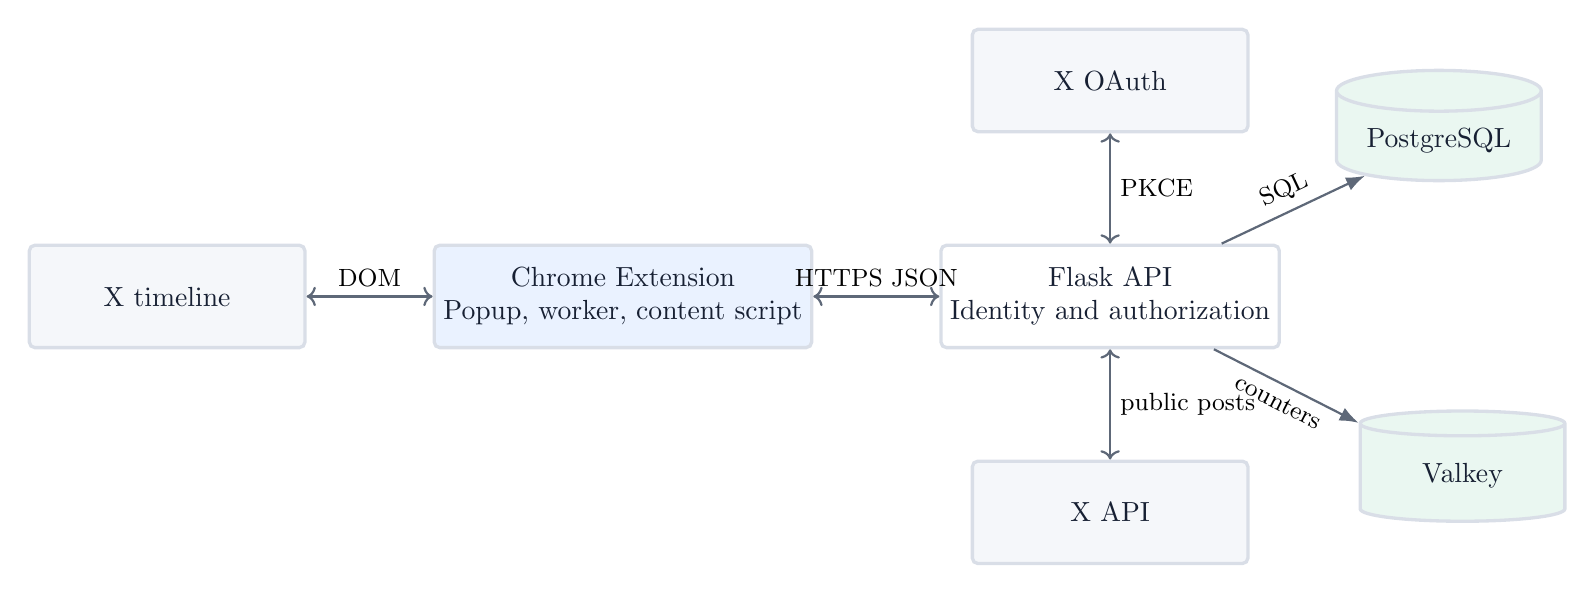
\begin{tikzpicture}[
  node distance=12mm and 16mm,
  box/.style={draw=Rule, very thick, rounded corners=2pt, fill=white,
    minimum width=35mm, minimum height=13mm, align=center, text=Ink},
  store/.style={draw=Rule, very thick, cylinder, shape border rotate=90,
    aspect=0.25, fill=SoftGreen, minimum width=26mm, minimum height=14mm,
    align=center, text=Ink},
  ext/.style={box, fill=SoftBlue},
  flow/.style={-{Latex[length=2.4mm]}, thick, draw=Muted}
]
  \node[ext] (chrome) {Chrome Extension\\Popup, worker, content script};
  \node[box, right=of chrome] (api) {Flask API\\Identity and authorization};
  \node[store, above right=8mm and 15mm of api] (db) {PostgreSQL};
  \node[store, below right=8mm and 15mm of api] (redis) {Valkey};
  \node[box, above=14mm of api, fill=CodeBg] (oauth) {X OAuth};
  \node[box, below=14mm of api, fill=CodeBg] (xapi) {X API};
  \node[box, left=of chrome, fill=CodeBg] (timeline) {X timeline};

  \draw[flow,<->] (chrome) -- node[above, font=\small]{HTTPS JSON} (api);
  \draw[flow] (api) -- node[above, sloped, font=\small]{SQL} (db);
  \draw[flow] (api) -- node[below, sloped, font=\small]{counters} (redis);
  \draw[flow,<->] (api) -- node[right, font=\small]{PKCE} (oauth);
  \draw[flow,<->] (api) -- node[right, font=\small]{public posts} (xapi);
  \draw[flow,<->] (chrome) -- node[above, font=\small]{DOM} (timeline);
\end{tikzpicture}
}
\caption{VisionX component architecture}
\label{fig:architecture}
\end{figure}

The extension never connects directly to PostgreSQL or the X API. The backend
is the policy enforcement point: it authenticates the viewer, checks the share,
resolves the owner's linked identity, applies caching, and normalizes the
upstream response. This keeps external API credentials and authorization rules
out of the browser.

\section{Repository Structure}
\begin{lstlisting}[style=visionx]
VisionX/
|-- backend/              Flask app, models, migration, tests
|-- extension/            Manifest V3 extension and JavaScript tests
|-- docs/                 Architecture, API, and project report
|-- scripts/              Validation and extension packaging
|-- .github/workflows/    Continuous integration
|-- docker-compose.yml    Local PostgreSQL, Valkey, and API
|-- render.yaml           Deployment blueprint
|-- README.md             Setup and operating guide
`-- LICENSE               MIT license
\end{lstlisting}

I used a monorepo because the API contract, popup behaviour, content renderer,
tests, and deployment configuration form one product. Keeping them together
makes interface changes visible and allows one continuous integration workflow
to validate the complete repository.

\section{Application Factory and Request Lifecycle}
The backend entry point is \code{create\_app} in
\code{backend/app/\_\_init\_\_.py}. Configuration is loaded before extensions
are initialized, and production startup validates the required environment.
The factory initializes SQLAlchemy, Alembic, Flask-Limiter, security headers,
and restricted CORS, then registers the route blueprints.

Each request is timed. The completion log records the method, path, status, and
duration. Known application errors, HTTP errors, and unexpected exceptions all
return JSON in a common shape. Database sessions are rolled back before an
error response when necessary, preventing a failed transaction from leaking
into subsequent work.

\chapter{Backend Implementation}

\section{Configuration and Service Boundaries}
The configuration class reads deployment values from environment variables.
There are no randomly generated production fallbacks for secrets. Startup
requires a database URL, JWT secret, cron secret, explicit allowed origins, and
a shared rate-limit storage URL. The JWT secret must contain at least
thirty-two characters, and a wildcard CORS origin is rejected.

SQLAlchemy engine options enable connection pre-ping and recycling, with pool
size and overflow controlled by environment values. PostgreSQL URLs are
normalized for the psycopg driver. Test configuration is separated so unit
tests can use an isolated database and memory-backed rate limiting.

Routes are grouped into blueprints for authentication, X accounts, shares,
feeds, health, and maintenance. X HTTP communication is kept in
\code{services/x\_api.py}; this made it possible to test upstream error and
normalization behaviour without placing request logic inside route handlers.

\section{VisionX Authentication}
Passwords are hashed with bcrypt using a configured work factor. Registration
validates username syntax, email structure, password length, uppercase and
lowercase characters, and at least one digit. Duplicate usernames and email
addresses are converted from database integrity errors into a stable conflict
response.

Successful registration or login returns two credentials:

\begin{itemize}
  \item a signed JWT access token with a short lifetime, subject identifier,
  username, token type, and unique token identifier;
  \item a high-entropy opaque refresh token whose SHA-256 digest, rather than
  raw value, is stored in the database.
\end{itemize}

The access token is checked by the \code{require\_auth} decorator. It validates
the signature, expiry, token type, subject, and current account state before
placing the user on Flask's request context.

\section{Refresh Token Rotation}
Refresh is implemented as rotation rather than repeated use of one long-lived
value. The backend selects the token record with a row lock, verifies that it
is active and unexpired, issues a replacement, revokes the presented record,
and links it to the replacement digest.

The replacement link also supports reuse detection. If a previously rotated
token appears again, the backend treats it as possible credential replay and
revokes every still-active refresh token for that user. The client must then
sign in again. Logout revokes the presented refresh token, while account
deletion removes the user and dependent records through database cascades.

\section{X OAuth Linking}
X account connection follows Authorization Code with PKCE. When linking starts,
the backend creates:

\begin{itemize}
  \item a random state value;
  \item a random PKCE verifier and its S256 challenge;
  \item a database record containing the state digest, verifier, user, and a
  short expiry.
\end{itemize}

Only the digest of state is used for callback lookup. The callback locks and
consumes the record before exchanging the authorization code. This ordering
makes the state single-use even if a later upstream call fails.

The exchanged token is used to call \code{/2/users/me}. VisionX accepts only a
public account and prevents the same X identity from being attached to two
VisionX accounts. It stores the X user identifier, username, display name,
profile image URL, and verification flag. The X user access token is not
written to the database. The requested scopes are limited to
\code{tweet.read} and \code{users.read}; \code{offline.access} is not
requested.

\section{Sharing Authorization}
A share is directional. In a row \code{owner\_id} identifies the user whose
linked feed may be viewed, while \code{shared\_with\_id} identifies the viewer.
The pair forms the primary key, preventing duplicate relationships.

The create route rejects invalid usernames, unknown or inactive accounts,
self-sharing, and duplicate access. Separate incoming and outgoing endpoints
make the user interface straightforward. Deletion is performed by the owner
and removes only that owner's grant.

The feed endpoint repeats authorization on the server. It does not trust the
popup's incoming list or a username supplied by the content script. A request
succeeds only if the owner exists, is active, has a linked X account, and has a
matching share row for the authenticated viewer.

\section{Public Feed Retrieval and Normalization}
The backend requests up to twenty-five posts from the owner's public user
timeline. Replies and reposts are excluded. The request asks for creation
information, entities, public metrics, media attachments, and media variants.
For video, the normalizer chooses the available MP4 variant with the highest
declared bit rate.

The normalized post contract is intentionally independent of the X response
layout. Each post includes:

\begin{itemize}
  \item post identifier, text, creation timestamp, and canonical X URL;
  \item a compact author object;
  \item reply, repost, like, quote, and view counts;
  \item a list of normalized media items.
\end{itemize}

This boundary protects the extension from changes in expansion arrays and
media-key joins. It also provides one place to apply defaults when an optional
metric or field is absent.

\section{Caching and Upstream Failure}
One \code{feed\_cache} row is maintained per owner. A valid cached response is
returned without contacting X and is marked with \code{cached: true}. An
expired or absent entry triggers retrieval and is replaced with normalized
posts and a new expiry. Disconnecting an X account removes its cached feed.

The cache reduces repeated external requests when several authorized viewers
select the same owner within a short period. It also makes the user experience
less sensitive to upstream latency. X rate-limit responses are translated into
a structured service error and preserve a \code{Retry-After} header. Network
exceptions, unsuccessful responses, and malformed JSON are handled as
upstream failures rather than unhandled server exceptions.

\section{Operational Routes}
\api{GET}{/health/live} proves that the Flask process can answer a request.
\api{GET}{/health/ready} additionally executes a simple database query.
Separating these checks allows a container platform to distinguish a running
process from an application that is ready to receive traffic.

The cleanup endpoint removes expired cache rows, OAuth states, and refresh
tokens. It is protected by a cron secret compared with
\code{secrets.compare\_digest}, which avoids an ordinary string comparison for
the shared secret.

\chapter{Database Design and Migration}

\section{Final Data Model}
\begin{longtable}{L{0.22\textwidth} L{0.30\textwidth} L{0.40\textwidth}}
\toprule
\textbf{Table} & \textbf{Important fields} & \textbf{Purpose} \\
\midrule
\endhead
\code{users} & username, email, password hash, status & Stores VisionX
identity and account state. \\
\code{feed\_shares} & owner ID, viewer ID & Represents the directional and
revocable authorization relationship. \\
\code{x\_accounts} & VisionX user ID, X user ID, public profile fields &
Stores a verified public X identity without an X user token. \\
\code{refresh\_tokens} & token digest, expiry, revocation, replacement digest
& Supports opaque refresh credentials, rotation, logout, and replay response. \\
\code{oauth\_link\_states} & state digest, PKCE verifier, expiry, used marker &
Supports a short-lived and single-use account-link operation. \\
\code{feed\_cache} & owner ID, posts JSON, fetch and expiry timestamps & Stores
the normalized public feed for a bounded period. \\
\bottomrule
\end{longtable}

\begin{figure}[htbp]
\centering
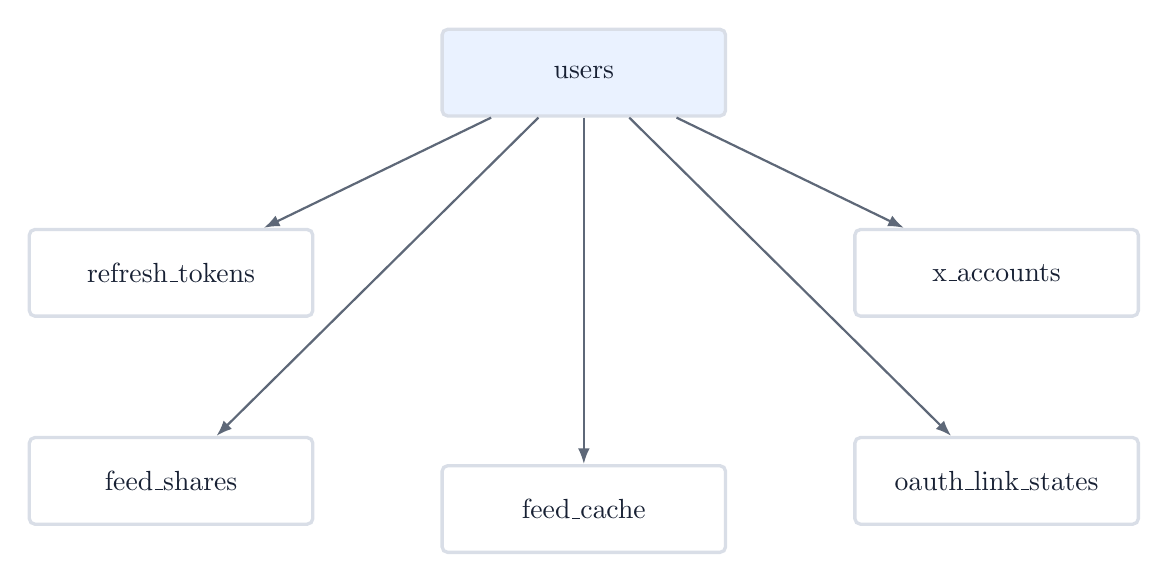
\begin{tikzpicture}[
  entity/.style={draw=Rule, very thick, rounded corners=2pt, fill=white,
    minimum width=36mm, minimum height=11mm, align=center, text=Ink},
  rel/.style={-{Latex[length=2mm]}, thick, draw=Muted}
]
  \node[entity, fill=SoftBlue] (users) {users};
  \node[entity, below left=14mm and 16mm of users] (refresh) {refresh\_tokens};
  \node[entity, below right=14mm and 16mm of users] (xaccount) {x\_accounts};
  \node[entity, below=15mm of refresh] (shares) {feed\_shares};
  \node[entity, below=15mm of xaccount] (oauth) {oauth\_link\_states};
  \node[entity, below=44mm of users] (cache) {feed\_cache};

  \draw[rel] (users) -- (refresh);
  \draw[rel] (users) -- (xaccount);
  \draw[rel] (users) -- (shares);
  \draw[rel] (users) -- (oauth);
  \draw[rel] (users) -- (cache);
\end{tikzpicture}
\caption{Simplified relational model}
\label{fig:data-model}
\end{figure}

Foreign keys use cascade deletion where dependent security or ownership data
must not outlive a user. Uniqueness constraints prevent duplicate usernames,
email addresses, X identities, token digests, state digests, and owner cache
rows. Indexes support account lookup, token ownership, and cache expiry.

\section{Legacy-Compatible Migration}
The initial Alembic migration is designed for two starting conditions: a fresh
PostgreSQL database and the earlier project schema. For a fresh installation it
creates the complete final model. For an existing installation it preserves
\code{users}, existing bcrypt password hashes, and valid
\code{feed\_shares}.

The migration removes the obsolete fetched-feed table and securely drops the
legacy cookie and token-derived tweet tables. Existing share relationships
remain, but a feed cannot return posts until its owner connects a verified
public X account. This is an intentional migration state: authorization can be
preserved without pretending that the old data source is still valid.

\chapter{Chrome Extension Implementation}

\section{Manifest V3 Configuration}
The extension uses Manifest V3 with an action popup, a background service
worker, an options page, and a content script for \code{https://x.com/*}. Its
base permissions are limited to \code{activeTab} and \code{storage}. It does
not request cookie, download, or general scripting permissions.

Local backend hosts are available for development. A deployed API origin is
requested as an optional host permission only when the user selects it in the
options page. The options validation requires HTTPS for non-local addresses
and stores only the origin.

\section{Background Service Worker}
\code{background.js} is the extension's network and session boundary. It stores
the access token, refresh token, and current user in extension-local storage,
while the selected API URL is kept in synchronized storage.

Popup code sends typed messages to the worker rather than duplicating fetch
logic. The worker attaches the access token, serializes JSON bodies, parses
structured responses, and converts network failure into a user-readable
backend connection error.

When an authenticated API request returns an unauthorized response, the worker
attempts one token rotation, saves both replacement credentials, and retries
the original request. A failed refresh clears local authentication so the
extension cannot remain in a misleading partially signed-in state.

\section{Popup Workflow}
The popup has loading, authentication, and dashboard views. Registration
performs immediate password and confirmation validation, while the backend
remains the final authority for all account rules.

After authentication, the dashboard shows VisionX identity, X connection
status, outgoing shares, and incoming feeds. The user can open X authorization
in a new tab, disconnect the account, create or revoke a share, load an
available feed, restore the original feed, log out, or delete the account.

Buttons and lists are built with DOM APIs. Empty lists have explicit states,
and a feed whose owner has not connected X is shown but cannot be loaded. The
popup checks that the active tab belongs to X before sending load or restore
messages and reports content-script communication failure instead of silently
doing nothing.

\section{Timeline Discovery and Injection}
X renders much of its page asynchronously. The content script first searches
for the primary timeline container. If it is not present, a
\code{MutationObserver} waits for a bounded interval. The observer disconnects
on success or timeout, preventing an unlimited page-wide watcher.

The renderer removes any previous VisionX container before inserting a new
one. It then deduplicates posts by identifier and prepends one section to the
timeline. Restoration removes that section by its unique identifier, so all
injected posts and the banner disappear together.

\section{Safe Post Rendering}
Post text, names, usernames, counts, and labels are assigned with
\code{textContent}. VisionX does not interpolate external data into HTML.
Media and post links pass through a URL parser that accepts only HTTPS.
External links use a new browsing context with \code{noopener noreferrer}.

Images are loaded lazily, video controls are enabled, and responsive CSS keeps
media inside the timeline width. The post grid changes avatar and spacing
dimensions on narrow screens. These choices keep the inserted content
recognizable inside X without copying private page state or altering the
original timeline nodes.

\chapter{End-to-End Workflows}

\section{Registration and Session Renewal}
\begin{enumerate}
  \item The popup submits registration data to the background worker.
  \item The worker sends the request to the Flask API.
  \item The backend validates the fields, hashes the password, and stores the
  user.
  \item The backend issues a JWT and opaque refresh token.
  \item The worker stores the credentials and the popup loads the dashboard.
  \item When the JWT expires, the worker rotates the refresh token and retries
  the interrupted API request.
\end{enumerate}

\section{Connecting an X Account}
\begin{figure}[htbp]
\centering
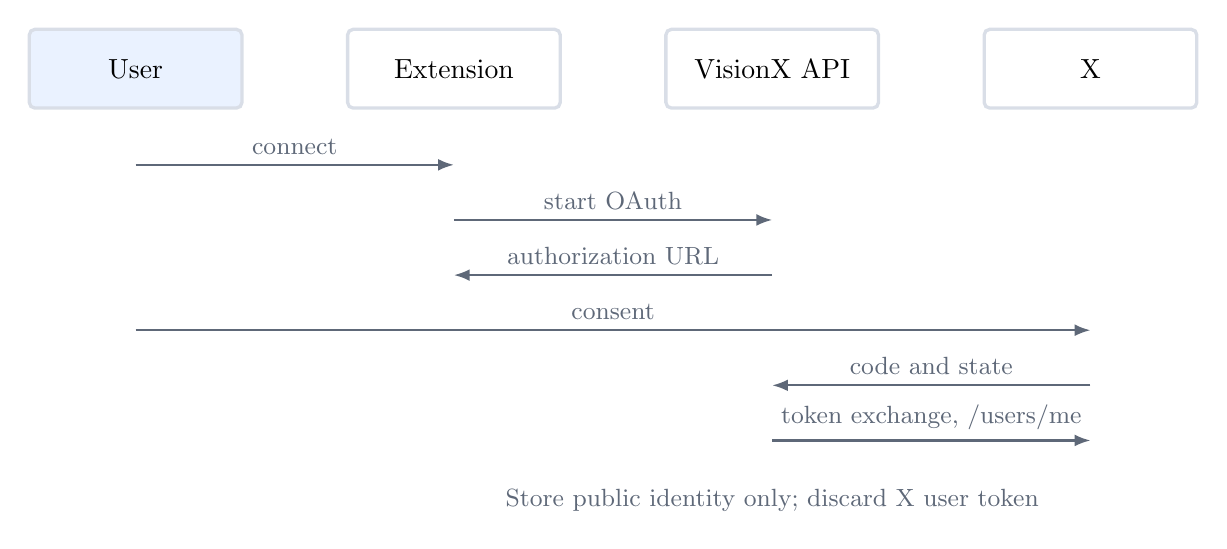
\begin{tikzpicture}[
  actor/.style={draw=Rule, very thick, rounded corners=2pt, fill=white,
    minimum width=27mm, minimum height=10mm, align=center},
  flow/.style={-{Latex[length=2mm]}, thick, draw=Muted},
  note/.style={font=\small, text=Muted, align=center}
]
  \node[actor, fill=SoftBlue] (user) {User};
  \node[actor, right=13mm of user] (ext) {Extension};
  \node[actor, right=13mm of ext] (api) {VisionX API};
  \node[actor, right=13mm of api] (x) {X};

  \draw[flow] ([yshift=-7mm]user.south) -- node[above,note]{connect} ([yshift=-7mm]ext.south);
  \draw[flow] ([yshift=-14mm]ext.south) -- node[above,note]{start OAuth} ([yshift=-14mm]api.south);
  \draw[flow] ([yshift=-21mm]api.south) -- node[above,note]{authorization URL} ([yshift=-21mm]ext.south);
  \draw[flow] ([yshift=-28mm]user.south) -- node[above,note]{consent} ([yshift=-28mm]x.south);
  \draw[flow] ([yshift=-35mm]x.south) -- node[above,note]{code and state} ([yshift=-35mm]api.south);
  \draw[flow] ([yshift=-42mm]api.south) -- node[above,note]{token exchange, /users/me} ([yshift=-42mm]x.south);
  \node[note, below=47mm of api] {Store public identity only; discard X user token};
\end{tikzpicture}
\caption{X account linking sequence}
\label{fig:oauth-flow}
\end{figure}

The state record binds the callback to the signed-in VisionX user who started
the flow. Because the callback consumes state before the external exchange, a
repeated callback cannot link again with the same state.

\section{Sharing and Loading a Feed}
\begin{enumerate}
  \item The owner enters another VisionX username and creates a share.
  \item The recipient sees the owner in the incoming-feed list.
  \item The recipient opens X and selects Load in the popup.
  \item The backend authenticates the recipient and checks the exact
  owner-to-recipient share.
  \item The backend returns a valid cache entry or retrieves and normalizes
  public authored posts from X.
  \item The popup sends the normalized posts to the active X tab.
  \item The content script discovers the timeline, renders one VisionX
  container, and confirms completion.
  \item Restore Original Feed removes the container without reloading or
  modifying X's own posts.
\end{enumerate}

\chapter{API Design}

\section{Response Conventions}
Protected endpoints require an Authorization header containing a bearer access
token. Application errors use one consistent envelope:

\begin{lstlisting}[style=visionx]
{
  "error": {
    "code": "machine_readable_code",
    "message": "Human-readable explanation."
  }
}
\end{lstlisting}

The machine-readable code lets the extension or a future client distinguish
states without parsing prose. Internal exception details are not returned in
production.

\section{Endpoint Summary}
\begin{longtable}{L{0.13\textwidth} L{0.34\textwidth} L{0.45\textwidth}}
\toprule
\textbf{Method} & \textbf{Path} & \textbf{Purpose} \\
\midrule
\endhead
POST & \code{/api/auth/register} & Create a VisionX account and issue a token
pair. \\
POST & \code{/api/auth/login} & Verify credentials and issue a token pair. \\
POST & \code{/api/auth/refresh} & Rotate a refresh token and issue a new
access token. \\
POST & \code{/api/auth/logout} & Revoke the supplied refresh token. \\
GET & \code{/api/auth/me} & Return the current profile and X connection. \\
DELETE & \code{/api/auth/account} & Delete the account after password
confirmation. \\
\midrule
POST & \code{/api/x/oauth/start} & Create state and PKCE data and return the X
authorization URL. \\
GET & \code{/api/x/oauth/callback} & Consume state, verify the public X
identity, and link it. \\
GET & \code{/api/x/account} & Return the current X connection status. \\
DELETE & \code{/api/x/account} & Disconnect X and clear the owner's cache. \\
\midrule
POST & \code{/api/shares} & Grant feed access to a VisionX username. \\
GET & \code{/api/shares/outgoing} & List viewers who can access the caller's
feed. \\
GET & \code{/api/shares/incoming} & List feeds available to the caller. \\
DELETE & \code{/api/shares/\{username\}} & Revoke an outgoing grant. \\
GET & \code{/api/feeds/\{username\}} & Return an authorized normalized public
feed. \\
\midrule
GET & \code{/health/live} & Report process liveness. \\
GET & \code{/health/ready} & Report application and database readiness. \\
POST & \code{/api/maintenance/cleanup} & Delete expired operational records
using the cron secret. \\
\bottomrule
\end{longtable}

\section{Feed Response}
A successful feed response contains the normalized posts, VisionX source user,
connected X username, fetch timestamp, cache indicator, and post count. The
explicit count is used by the popup's completion message, while the cache
indicator supports diagnostics without changing the rendered post contract.

\chapter{Security and Privacy}

\section{Credential Handling}
VisionX keeps three credential types separate:

\begin{itemize}
  \item password hashes are stored with bcrypt and raw passwords are never
  logged;
  \item VisionX access tokens are short-lived, while only refresh-token digests
  are stored server-side;
  \item the X user token exists only during the linking request and is
  discarded after identity verification.
\end{itemize}

The X application bearer token, OAuth client secret, JWT secret, and cron
secret are environment values. Example configuration contains placeholders,
not deployable credentials.

\section{Authorization and Input Boundaries}
Authentication alone does not grant feed access. The share check is performed
inside the feed route using database identifiers for both owner and viewer.
Username validation, self-share rejection, unique constraints, and account
state checks cover the main invalid relationship cases.

The extension treats backend and X content as external input. It validates
backend URLs, sends API requests through one worker, uses structured JSON, and
constructs timeline elements through DOM APIs. HTTPS-only URL validation is
applied separately from text rendering.

\section{Platform and Browser Controls}
Restricted CORS permits only configured origins. Flask-Talisman adds security
headers, and production deployment can enforce HTTPS and strict transport
security. API limits are shared through Valkey so counters remain effective
across multiple Gunicorn workers.

Manifest permissions were deliberately reduced. The extension has no cookie
permission and no broad always-on production host access. A user must grant
the selected deployed backend origin through the options flow.

\section{Data Retention}
Durable data consists of VisionX account information, explicit sharing
relationships, public X identity fields, token digests, and the bounded feed
cache. Expired OAuth state, refresh records, and cache rows are removed through
maintenance. Disconnecting X deletes the linked identity and cached feed;
deleting a VisionX account cascades through its dependent records.

\chapter{Testing and Validation}

\section{Backend Test Coverage}
The backend test suite contains twenty tests covering:

\begin{itemize}
  \item registration validation, login, profile access, and account deletion;
  \item access-token handling, refresh rotation, logout, and refresh-token
  replay response;
  \item OAuth state expiry and reuse, X identity linking, duplicate identity,
  and rejection of protected accounts;
  \item creation, listing, authorization, and revocation of shares;
  \item feed caching, X rate limits, malformed or failed upstream responses,
  and normalized post content;
  \item liveness, database readiness, maintenance authentication, configuration
  validation, and migration from the earlier schema.
\end{itemize}

The tests run against an isolated application configuration. The continuous
integration workflow additionally provides PostgreSQL and Valkey services,
runs the Alembic upgrade, and executes the suite with coverage reporting.

\section{Extension Test Coverage}
The JavaScript suite contains eleven tests using Node's test runner and JSDOM.
It checks:

\begin{itemize}
  \item safe URL filtering, count formatting, post construction, duplicate
  removal, and complete feed restoration;
  \item delayed timeline discovery and timeout behaviour;
  \item background response parsing, token storage, renewal, and clearing;
  \item popup registration validation, active-tab checks, and message failure
  handling.
\end{itemize}

ESLint and Prettier checks enforce consistent JavaScript quality. The manifest
is parsed as JSON during continuous integration, and the packaging script
builds a distributable archive from a controlled file set.

\section{Repository and Runtime Validation}
The completed repository was checked with the following layers:

\begin{longtable}{L{0.28\textwidth} L{0.62\textwidth}}
\toprule
\textbf{Check} & \textbf{Observed result} \\
\midrule
\endhead
Python quality & Ruff lint and format checks completed successfully. \\
Backend tests & Twenty automated tests passed. \\
Extension quality & ESLint and Prettier checks completed successfully. \\
Extension tests & Eleven automated tests passed. \\
Dependency audit & Python and npm audits reported no applicable known
vulnerabilities at the configured threshold. \\
Migration & Fresh and legacy-compatible migration paths were exercised. \\
Containers & PostgreSQL, Valkey, and the API started together; liveness and
readiness returned successful responses. \\
Image review & The backend container was checked for a non-root runtime and a
restricted build context. \\
Extension package & The archive was built and its manifest and expected files
were verified. \\
Interface review & The popup was rendered at extension dimensions and its
authentication views, dashboard states, and text fit were inspected. \\
\bottomrule
\end{longtable}

During interface validation I found a form visibility issue caused by CSS
overriding the HTML \code{hidden} state. I corrected the visibility rule and
rechecked both login and registration views. This was a useful reminder that a
passing DOM test does not replace looking at the rendered interface.

\section{Credential-Dependent Verification}
OAuth and feed HTTP behaviour are covered with controlled responses in the
automated tests. A genuine X authorization and public feed retrieval still
require approved developer credentials, a registered callback, and an
available X API plan. Those live calls are therefore a deployment acceptance
step, not something I claim as completed by the local test suite.

\chapter{Deployment and Release Readiness}

\section{Docker Compose}
The local Compose environment starts PostgreSQL, Valkey, and the backend. Both
supporting services have health checks, and the backend waits for healthy
dependencies. Migrations run as part of backend startup before Gunicorn serves
requests.

The backend image installs pinned requirements, copies only the application
and migration files needed at runtime, and runs as an unprivileged user. The
\code{.dockerignore} excludes local environments, caches, tests, and secrets
from the build context.

\section{Render Blueprint}
The deployment blueprint defines:

\begin{itemize}
  \item a PostgreSQL database;
  \item a private Redis-compatible key-value service for distributed limits;
  \item a Docker web service with a readiness health check;
  \item a pre-deploy Alembic upgrade;
  \item generated VisionX secrets and manually supplied X credentials and
  origins.
\end{itemize}

The blueprint is configuration, not evidence of a live deployment. Before
deployment, the X callback and extension origin must be registered exactly and
the production API URL must be selected in the extension options.

\section{Continuous Integration}
The GitHub Actions workflow has separate backend, extension, and Docker jobs.
The backend job installs development requirements, checks Ruff formatting,
applies migrations, runs tests, and audits Python packages. The extension job
installs locked Node dependencies, runs linting, formatting, tests, manifest
validation, the npm audit, and packaging. The Docker job confirms that the
backend image builds from a clean checkout.

\section{Environment Contract}
\begin{longtable}{L{0.31\textwidth} L{0.59\textwidth}}
\toprule
\textbf{Variable} & \textbf{Purpose} \\
\midrule
\endhead
\code{DATABASE\_URL} & PostgreSQL connection used by SQLAlchemy and Alembic. \\
\code{JWT\_SECRET} & Access-token signing secret. \\
\code{CRON\_SECRET} & Authentication value for maintenance cleanup. \\
\code{X\_CLIENT\_ID} & OAuth application identifier. \\
\code{X\_CLIENT\_SECRET} & OAuth confidential-client secret. \\
\code{X\_BEARER\_TOKEN} & Application credential for public post retrieval. \\
\code{X\_REDIRECT\_URI} & Exact callback registered with X. \\
\code{ALLOWED\_ORIGINS} & Explicit comma-separated trusted extension origins. \\
\code{RATELIMIT\_STORAGE\_URI} & Redis-compatible shared limit storage. \\
\bottomrule
\end{longtable}

\chapter{Limitations and Future Work}

\section{Current Limitations}
\begin{itemize}
  \item VisionX supports public accounts only. A protected account is rejected
  because the application deliberately avoids retaining delegated user access.
  \item The public timeline request returns a bounded recent set rather than a
  paginated history.
  \item Replies and reposts are excluded and there is no extension control to
  change that filter.
  \item The content script depends on an X timeline selector. The bounded wait
  prevents hanging, but a substantial X page-structure change may require a
  selector update.
  \item The system uses one application bearer token, so X project limits apply
  across all VisionX users.
  \item The project does not include a separate website or administrative
  console.
\end{itemize}

\section{Future Enhancements}
The next useful improvement would be pagination with a small cursor-based
interface so a viewer can request older posts without increasing the first
response. I would also add optional owner-controlled filters for replies,
reposts, and media while keeping the server as the source of authorization.

For operations, metrics for cache hit rate, upstream latency, token reuse
events, and feed failures would make production behaviour easier to assess.
These metrics should avoid usernames and post text. A small administrative
view could expose aggregate service health without providing access to user
feeds.

The extension could support Firefox after testing the background and optional
permission differences. Accessibility testing can also be expanded with
keyboard-only walkthroughs and automated contrast and naming checks.

Finally, a live integration test environment could be added if stable X test
credentials and suitable API access are available. Such a test should remain
separate from pull-request checks to avoid exhausting external limits.

\chapter{Conclusion}
VisionX demonstrates a complete browser-extension and web-service workflow
rather than an isolated interface prototype. A VisionX user can create an
account, verify a public X identity, grant another user access, and allow that
viewer to load normalized public posts inside X. The recipient can restore the
original timeline without a page rewrite.

The most important implementation decision was to keep X session material out
of the extension and database. OAuth is used for identity verification, the X
user token is discarded, and feed retrieval is performed through the official
public API. Combined with server-side share checks, rotating VisionX sessions,
restricted browser permissions, safe DOM rendering, and bounded caching, this
gives the project a clear security and privacy model.

The repository also contains the less visible work needed for a credible final
project: a legacy-compatible migration, structured failures, health checks,
container orchestration, deployment configuration, automated tests,
dependency audits, extension packaging, and technical documentation. Live X
credentials remain an external deployment requirement, but the application
and its release pipeline are prepared for that final integration step.

\appendix
\chapter{Local Operating Procedure}

\section{Starting the Backend}
\begin{lstlisting}[style=visionx]
cp backend/.env.example backend/.env
# Fill the required secrets and X application credentials.
docker compose up --build
\end{lstlisting}

The API listens on the configured local port. The readiness route should be
checked before loading the extension.

\section{Loading the Extension}
\begin{enumerate}
  \item Open the browser's extension management page and enable developer mode.
  \item Choose Load unpacked and select the repository's \code{extension}
  directory.
  \item Open VisionX options and confirm the backend URL.
  \item Add the extension origin to \code{ALLOWED\_ORIGINS} and restart the API.
  \item Register the exact X callback URL in the X developer application.
\end{enumerate}

\section{Project Repository}
The complete source repository is available at:

\begin{center}
\url{https://github.com/nayvirmis/VisionX}
\end{center}

\chapter{References}
\begin{thebibliography}{9}

\bibitem{xpolicy}
X Developer Platform,
\emph{Developer Policy}.
\url{https://docs.x.com/developer-terms/policy}

\bibitem{xoauth}
X Developer Platform,
\emph{OAuth 2.0 Authorization Code Flow with PKCE}.
\url{https://docs.x.com/fundamentals/authentication/oauth-2-0/authorization-code}

\bibitem{xtimeline}
X Developer Platform,
\emph{User Post Timelines}.
\url{https://docs.x.com/x-api/posts/timelines/introduction}

\bibitem{chrome}
Chrome for Developers,
\emph{Chrome Extensions and Manifest V3}.
\url{https://developer.chrome.com/docs/extensions/}

\bibitem{flask}
Pallets Projects,
\emph{Flask Documentation}.
\url{https://flask.palletsprojects.com/}

\bibitem{sqlalchemy}
SQLAlchemy,
\emph{SQLAlchemy Documentation}.
\url{https://docs.sqlalchemy.org/}

\bibitem{alembic}
SQLAlchemy,
\emph{Alembic Documentation}.
\url{https://alembic.sqlalchemy.org/}

\end{thebibliography}

\end{document}
